\chapter{Marco teórico}
\label{chap:background}

% En este capítulo se definen los conceptos teóricos y formulaciones matemáticas que sustentan las metodologías y experimentos computacionales realizados en esta investigación.

Todo se escribe en texto normal, salvo cuando se escriben \textit{nuevos conceptos} (también pueden escribirse en \textbf{negritas}). Es importante elegir formatos de texto adecuados a variables matemáticas como $x$ o computacionales como tipos de archivo \texttt{CSV}.

También se puede citar autores con \citet{arias2006} y su referencia bibliográfica mediante \cite{arias2006}. Además, puedes agregar conceptos secundarios en notas de pie\footnote{Ejemplo de nota al pie.}.

Así se ponen ecuaciones
\begin{equation}
J(c_j) = \sum_{x_i \in c_j} \lVert x_i - \mu_j \rVert ^2.
\end{equation}

De este modo se enumeran elementos
\begin{enumerate}
    \item Elemento 1,
    \item elemento 2,
    \item elemento 3.
\end{enumerate}

Y así se hacen listas desordenadas
\begin{itemize}
    \item Elemento 1,
    \item elemento 2,
    \item elemento 3.
\end{itemize}

Si lo necesitas, puedes agregar algoritmos
\begin{algorithm}
    \caption{Algoritmos en \url{https://tex.stackexchange.com/a/146053}.}
    \SetAlgoLined
    \ForEach{archivo en carpetas}{
      \ForEach{página en archivo}{
        \If{página contiene 'fin'}{
          cerrar página\;
        }
      }
      exportar datos en \texttt{CSV}\;
    }
    \label{alg}
\end{algorithm}

Por último, es posible incluir cuadros, como el que aparece en \ref{cuadro} (con todo y su página de aparición, o sea: \pageref{cuadro}), así como la imagen \ref{figura} (en la p. \pageref{figura}).

\begin{table}[]
  \caption{Generador en \url{http://www.tablesgenerator.com/latex_tables}}
  \centering
  \label{cuadro}
  \begin{tabular}{lll}
  Columna 1 & Columna 2 & Columna 3 \\
  Dato 1    & Dato 2    & Dato 3    \\
  Dato 4    & Dato 5    & Dato 6   
  \end{tabular}
\end{table}

\begin{figure}
  \caption{Figura de ejemplo.}
  \centering
  \label{figura}
  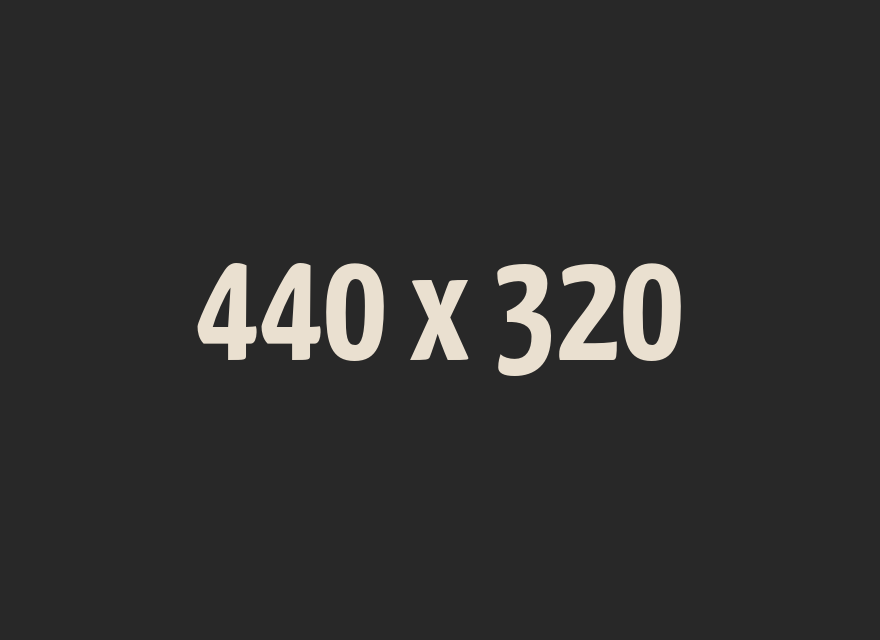
\includegraphics[width=\textwidth]{ejemplo}
\end{figure}
